\section{Experiments}

\begin{table}[!h]
	\centering
	\begin{tabular}{|c||c|c|c|c|} \hline
		Data split & Source & Segmented & Images & Patients \\\hline
		Training & \vtop{\hbox{\strut Med-Seg}\hbox{\strut ICTCF}}&
		\vtop{\hbox{\strut Yes}\hbox{\strut No}} & 
		\vtop{\hbox{\strut 698}\hbox{\strut 6654}}&
		\vtop{\hbox{\strut 39}\hbox{\strut 1338}}\\\hline
		Validation & Med-Seg & Yes & 114 & 35 \\\hline
		Testing & Med-Seg & Yes & 117 & 35 \\\hline
	\end{tabular}
	\caption{This table shows the data distribution between the datasets that we use to evaluate our model on. Med-Seg refers to the COVID-19 CT Segmentation data set and ICTCF refers to the ICTCF data set.}
	\label{tab:dataset}
\end{table}

\begin{table*}[!h]
	\centering
	\begin{tabular}{| c | c || c c c c c | c ||}
		\hline
		Methods & & Dice & Jaccard & Sen. & Spec. & MAE & AUC \\ \hline
		Single SInfNet &  Mean & \textbf{0.36} & \textbf{0.27} & \textbf{0.58} & 0.9491 & 14.43 & \textbf{0.9909} \\ \cline{2-7}
		& Error & $\pm$ 0.058 & $\pm$ 0.047 & $\pm$0.084 & $\pm$ 0.015 & $\pm$ 0.77 & \\ \hline
		Single SInfNet + data aug(0.4) &  Mean & 0.32 & 0.24 & 0.54 & \textbf{0.9562} & 16.31 & 0.9903 \\ \cline{2-7}
		& Error & $\pm$0.056  & $\pm$0.046  &$\pm$\textbf{0.082} &$\pm$\textbf{0.015} &$\pm$0.90 & \\ \hline
		Single SInfNet + data aug (0.5) &  Mean & 0.34 & 0.25 & 0.56 & 0.9474 & 14.67 & 0.9893 \\ \cline{2-7}
		& Error &$\pm$0.058 &$\pm$0.048 &$\pm$0.084 &$\pm$0.016 & $\pm$0.82 & \\ \hline \hline
		Single Self-SInfNet &  Mean & 0.31 & 0.24 & 0.51 & 0.9299 & 16.08 & 0.9883  \\ \cline{2-7}
		& Error & $\pm$0.057 & $\pm$0.047 &$\pm$0.083  & $\pm$0.023 & $\pm$ \textbf{0.72} & \\ \hline
		Single Self-SInfNet + data aug &  Mean & 0.28 & 0.20 & 0.49 & 0.9450 &  \textbf{14.26} & 0.9795 \\ \cline{2-7}
		& Error & $\pm$ \textbf{0.054}  & $\pm$ \textbf{0.042} & $\pm$ 0.083 & $\pm$0.019 & $\pm$0.75 & \\ \hline
	\end{tabular}
	\caption{Quantitative result for comparison between Single segmentation InfNet and self-supervised single segmentation InfNet in the test set.}
	\label{tab:single}
\end{table*}

\begin{table*}[!h]
	\centering
	\small
	\begin{tabular}{| c | c || c c c c c | c || c c c c c | c |}
		\hline
		& &\multicolumn{6}{c||}{Ground-Glass Opacity} & \multicolumn{6}{c|}{Consolidation}\\ \cline{3-14}
		Methods & & Dice & Jac & Sen. & Spec. & MAE & AUC & Dice & Jac & Sen. & Spec. & MAE & AUC \\\hline
		SInfNet & Mean & \textbf{0.34} & \textbf{0.24} & \textbf{0.41} & 0.9936 & 0.010 & \textbf{0.86} & \textbf{0.18} & \textbf{0.14}  & \textbf{0.20} & 0.9976 & 0.006 & \textbf{0.75}  \\ \cline{2-14}
		& Error & $\pm$0.052 & $\pm$0.040 & $\pm$0.067 & $\pm$0.003 & $\pm$0.004 & & $\pm$0.055 & $\pm$0.047 & $\pm$0.061 & $\pm$ 0.001 & $\pm$0.003 & \\ \hline \hline
		
		\vtop{\hbox{\strut SInfNet+}\hbox{\strut data aug(0.4)}} & Mean & 0.31 & 0.22 & 0.38 & 0.9939 & 0.009 & 0.87 & 0.15 & 0.11 & 0.17 & 0.9944 & 0.009 & 0.73  \\ \cline{2-14}
		& Error & $\pm$ 0.053 & $\pm$0.042  & $\pm$0.067 & $\pm$0.003 & $\pm$\textbf{0.003} & & $\pm$0.048 & $\pm$0.039 & $\pm$\textbf{0.055} & $\pm$0.002 & $\pm$0.004 & \\ \hline \hline
		
		\vtop{\hbox{\strut SInfNet+}\hbox{\strut data aug(0.5)}} & Mean & 0.31 & 0.22 & 0.37 & 0.9931 & 0.010 & 0.86 & 0.15 & 0.11 & 0.15 & 0.9981 & 0.006 & 0.70 \\ \cline{2-14}
		& Error & $\pm$ 0.052 & $\pm$ 0.041 & $\pm$ 0.065 & $\pm$0.003 & $\pm$0.004 & & $\pm$0.050 & $\pm$0.042 & $\pm$0.055 & $\pm$0.001 & $\pm$0.004 & \\ \hline \hline
		
		\vtop{\hbox{\strut SSInfNet}\hbox{\strut }} & Mean & 0.30 & 0.21 & 0.33 & \textbf{0.9947} & \textbf{0.009} & 0.83 & 0.16 & 0.12 & 0.17 & 0.9985 & \textbf{0.005} & 0.72  \\ \cline{2-14}
		& Error & $\pm$0.052 & $\pm$0.040 & $\pm$0.062 & $\pm$0.003 & $\pm$0.004 & & $\pm$0.053 & $\pm$0.046 & $\pm$0.059 & $\pm$0.001 & $\pm$\textbf{0.003} &  \\ \hline \hline
		
		\vtop{\hbox{\strut SSInfNet+}\hbox{\strut data aug}} & Mean & 0.30 & 0.21 & 0.33 & 0.9928 & 0.01 & 0.83 & 0.12 & 0.09 & 0.15 & \textbf{0.9988} & 0.01 & 0.61 \\ \cline{2-14}
		& Error & $\pm$\textbf{0.051} & $\pm$\textbf{0.039} & $\pm$0.062 & $\pm$0.003 & $\pm$0.004 & & $\pm$\textbf{0.045} & $\pm$\textbf{0.037} & $\pm$0.056 & $\pm$\textbf{0.001} & $\pm$0.004 & \\ \hline \hline
	\end{tabular}
	\caption{Quantitative result of Ground-glass Opacities \& Consolidation on the test data set. Prior is obtained from the single segmentation InfNet}
	\label{tab:multi-weakprior}
\end{table*}

\begin{table*}[!h]
	\centering
	\small
	\begin{tabular}{| c | c || c c c c c | c || c c c c c | c |}
		\hline
		& &\multicolumn{6}{c||}{Ground-Glass Opacity} & \multicolumn{6}{c|}{Consolidation}\\ \cline{3-14}
		Methods & & Dice & Jac & Sen. & Spec. & MAE & AUC & Dice & Jac & Sen. & Spec. & MAE & AUC \\\hline
		SInfNet & Mean & 0.61 & \textbf{0.57} & 0.61 & 0.9970 & 0.004 & 0.96 & \textbf{0.21} & 0.17 & \textbf{0.22} & 0.9991 & 0.004 & 0.80 \\ \cline{2-14}
		& Error & $\pm$0.078 & $\pm$0.075 & $\pm$0.078 & $\pm$0.002 & $\pm$0.003 & & $\pm$0.061 & $\pm$0.054 & $\pm$0.067 & $\pm$0.0004 & $\pm$0.002 & \\ \hline \hline
		
		\vtop{\hbox{\strut SInfNet+}\hbox{\strut data aug(0.4)}} & Mean & 0.60 & 0.56 & 0.61 & 0.9965 & 0.004 & \textbf{0.98} & 0.20 & \textbf{0.17} & 0.21 & \textbf{0.9996} & 0.004 & 0.76 \\ \cline{2-14}
		& Error & $\pm$0.079 & $\pm$0.078 & $\pm$0.081 & $\pm$0.003 & $\pm$0.003 & & $\pm$0.060 & $\pm$0.052 & $\pm$0.065 & $\pm$\textbf{0.0002} & $\pm$0.003 &  \\ \hline \hline
		
		\vtop{\hbox{\strut SInfNet+}\hbox{\strut data aug(0.5)}} & Mean & 0.61 & 0.57 & \textbf{0.62} & 0.9964 & 0.004 & 0.97 & 0.19 & 0.16 & 0.20 & 0.9995 & 0.004 & 0.76 \\ \cline{2-14}
		& Error & $\pm$0.078 & $\pm$0.077 & $\pm$0.081 & $\pm$0.003 & $\pm$0.003 & & $\pm$0.060 & $\pm$0.052 & $\pm$0.065 & $\pm$0.0002 & $\pm$0.003 & \\ \hline \hline

		SSInfNet & Mean & 0.60 & 0.56 & 0.61 & \textbf{0.9974} & \textbf{0.003} & 0.96 & 0.20 & 0.16 & 0.22 & 0.9991 & \textbf{0.003} & 0.83 \\ \cline{2-14}
		& Error & $\pm$0.077 & $\pm$0.075 & $\pm$0.078 & $\pm$\textbf{0.002} & $\pm$\textbf{0.002} & & $\pm$0.061 & $\pm$0.054 &$\pm$0.068 & $\pm$0.0005 &$\pm$\textbf{0.002} &  \\ \hline \hline
		
		\vtop{\hbox{\strut SSInfNet+}\hbox{\strut data aug}}& Mean & 0.57 & 0.52 & 0.58 & 0.9967 & 0.004 & 0.97 & 0.19 & 0.15 & 0.20 & 0.9994 & 0.004 & \textbf{0.87} \\ \cline{2-14}
		& Error & $\pm$\textbf{0.075} & $\pm$\textbf{0.071} & $\pm$\textbf{0.076} & $\pm$0.003 & $\pm$0.003 & & $\pm$\textbf{0.058} & $\pm$\textbf{0.050} & $\pm$\textbf{0.064} & $\pm$0.0003 & $\pm$0.002 & \\ \hline \hline
	\end{tabular}
	\caption{Quantitative result of Ground-glass Opacities \& Consolidation on the test data set. Prior is obtained from the test set.}
	\label{tab:multi-strongprior}
\end{table*}


\subsection{Datasets}
The dataset that we will be using is an integrative resource of chest computed tomography images and clinical features of patients with COVID-19 pneumonia (ICTCF) \cite{ref23} which contains the severity score for each CT lung image and CT lung images from medical segmentation website \cite{ref26}. 

ICTCF contains 127 types of clinical features and laboratory confirmed cases of COVID-19 from 1170 patients including the severity for the CT lung images. However, ICTCF dataset does not contain the segmentation labels for the ground-glass opacities and the consolidation in the CT lung images. In total, there are 6654 of CT lung images in ICTCF dataset. Originally, there were 1521 patients. However, some of the patients are missing CT lung images. We remove these patients that are missing CT lung images. After preprocessing the patients, the dataset was left with 1338 patients that contains CT lung images. The dataset can be found here: http://ictcf.biocuckoo.cn/. 

As for the medical segmentation dataset, they contain ground truth label for the segmentation for ground-glass opacities and consolidation of the CT lung images but does not contain the severity score for the CT Lung images. The total amount of CT lung images contain in medical segmentation dataset is 932 CT lung images. We randomly assign the CT lung images into training set, validation set, and testing set of which the training set contains 698 CT lung images, the validation set contains 114 CT lung images, and the testing set contains 117 CT lung images. 

The assignment of the dataset can be seen in \ref{tab:dataset}.


\begin{figure}
	\centering
	\small
	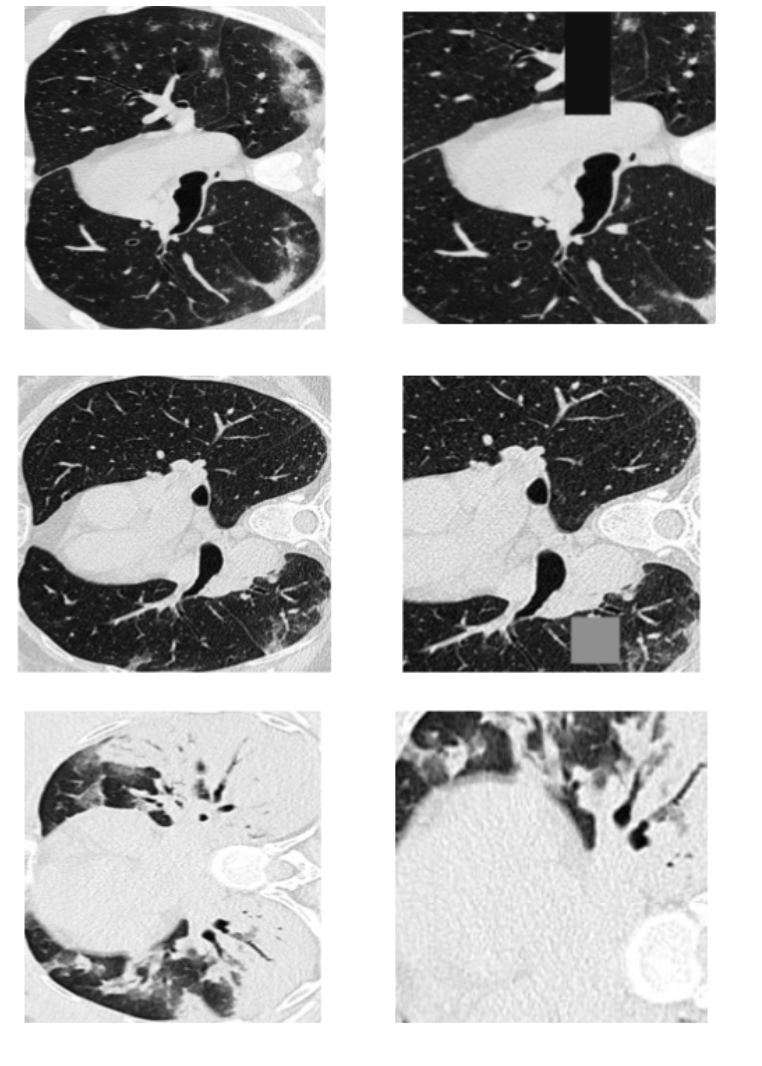
\includegraphics[width=\linewidth]{data_aug.png}
	\caption{Example of data augmentation on the CT lung images.}
	\label{fig:data_aug}
\end{figure}

\subsection{Experimental Settings}
During the self-supervised image inpainting stage, we train the network for 2000 epochs. The network is trained for the first 200 epochs before we train the coach network for 200 epochs which increases the complexity of the masks generated. After that, we alternate in between training the self-supervised image inpainting and the coach network with 100 epochs in between. For every alternating between the training of the self-supervised image inpainting and the coach network, we set the learning rate to 0.1 at the start of the epoch, we set the learning rate to 0.01 at 40th epoch, we set the learing rate to 0.001 at 80th eochs, and 0.0001 at the 90th epoch.  We use SGD as the optimizer for the self-supervised image inpainting.  We set the momentum to 0.9 and the weight decay to 0.0005. As for the optimizer for the coach network, we use Adam optimizer with learning rate of 0.00001.

For the Single InfNet, we train the network for 500 epochs. We use Adam as the optimizer with learning rate of 0.0001. 

For the Multi InfNet, we train the network for 500 epochs. We use SGD as the optimizer. The momentum is set as 0.7 and the learning rate is set as 0.01.

For the severity score calculation, there are several different labels obtained from ICTCF dataset for severity, The different severity are: \textit{Regular, Mild, Control, Severe, Critically ill.}  The assign the different labels with score ranging from 0 to 2. \textit{Regular, Mild, and Control} are assign having a severity score of 0. \textit{Severe} is assign having a severity score of 1. \textit{Critically ill} is assign having a severity score of 2. We use the metrics provided by sklearn to caclulate the F1 Score, Precision Score, and Recall Score for the severity score prediction. We use 'micro' as the averaging for the scores as provided by sklearn.

\subsection{Data Augmentation}
We used data augmentation to increase our data samples size. The data agumentation that we used includes \textit{vertical flipping, horizontal flipping, random crop, and random cutout}. For the random cutout percentage, we experimented that 0.5 cDuring tutout of the CT lung images yield higher performance than the rest of the value. This is because entropy at 0.5 is the highest which could increase more variability of the images. Examples of the data augmentation can be seen in figure \ref{fig:data_aug}.
The left column is the original CT lung images while the right column is the augmented CT lung images. The first row involves random cropping and random cutout. The second row involves random cropping and random cutout. The third row involves random cropping and vertical flipping. The random cutout involves patching the image with colors of the same value of rgb. For instance, if the value of r is 10, then the value of g and b are also 10. If the value of r is 50, then the value of g and b are also 50.

